\documentclass[11pt]{article}
\usepackage[margin=1in]{geometry}
\usepackage[T1]{fontenc}
\usepackage{lmodern,microtype,amsmath,amssymb,amsthm,mathtools,booktabs,graphicx,xcolor}
\usepackage{enumitem}
\usepackage[numbers,sort&compress]{natbib}
\usepackage[colorlinks=true,allcolors=blue!55!black]{hyperref}
\usepackage{xurl}
\graphicspath{{figures/}{../figures/}}
\setlist{nosep}
\setlength{\emergencystretch}{2em}
\newtheorem{theorem}{Theorem}
\newtheorem{proposition}[theorem]{Proposition}
\newtheorem{lemma}[theorem]{Lemma}
\newtheorem{corollary}[theorem]{Corollary}
\newcommand{\E}{\mathbb E}
\newcommand{\R}{\mathbb R}
\newcommand{\ind}{\mathbf 1}
\newcommand{\Var}{\operatorname{Var}}
\newcommand{\clip}{\operatorname{clip}}
\newcommand{\norm}[1]{\left\lVert#1\right\rVert}
\title{The Audit Complexity of Group-Relative Policy Updates}
\author{Shengwei Zhang\\University of Pennsylvania}
\date{September 12, 2026}
\begin{document}
\maketitle
\begin{abstract}
Scaling agent training requires deciding which expensive terminal outcomes to verify. For group-relative policy optimization, this is a nonlinear estimation problem: unbiased reward estimates need not yield unbiased normalized advantages, and unbiased advantages need not preserve a clipped objective. We study the conditional target obtained by completely verifying a fixed binary-reward group. For any nonconstant fixed score vector, we prove that an unclipped group-normalized update has Boolean degree $G-1$ for even group size $G$ and $G-2$ for odd $G$. Each sign-separated advantage has degree $G$ for even $G$ and $G-1$ for odd $G$. These identities give sharp worst-case query-depth obstructions to pointwise unbiased estimation under a hard audit cap. Under an expected budget, we instantiate randomized telescoping on positive and negative advantage coefficients, preserving the complete-label clipped surrogate at every fixed parameter value. Independent-Bernoulli completion admits exact count-based calculations and a model-based monotone survival schedule. Exact enumeration, a controlled estimation study, and 180 runs of constructed stateful policy training examine both validity and efficiency. Sequential correction approaches full-verification performance using roughly half the training queries in the constructed tasks, but does not establish an advantage over whole-group residual correction and takes more local computation. Charging development-label costs eliminates every apparent advantage of a tuned schedule in the initial 135-setting comparison. A frozen-model diagnostic on 49 historical software-task groups gives lower mean projected error for model-derived schedules, with broad pointwise intervals and no on-policy inference. The results identify the function that must be audited, distinguish exact unbiasedness from useful approximation, and expose when a simple whole-group audit is the appropriate baseline.
\end{abstract}

\section{Introduction}
A long-running agent can appear to finish a task while leaving a prerequisite unsatisfied. A software repair may pass a visible check but fail a broader test suite; a multi-stage release can update its final artifact while retaining stale dependency metadata. Obtaining a stronger terminal verdict may require executing tests, inspecting state, or applying a more expensive verifier. As the number and diversity of training environments increase, checking every rollout can become a substantial part of data collection. This motivates a specific question: given a fixed collection of trajectories and cheap predictions, which reference-verifier queries are sufficient to reconstruct the intended training update?

The question differs from improving a verifier's classification accuracy. Group Relative Policy Optimization (GRPO) standardizes rewards within a rollout group \citep{shao2024}. The resulting update depends jointly on multiple outcomes. An inverse-probability correction that is valid for individual rewards need not survive division by the group's estimated standard deviation. PPO-style clipping adds a second nonlinearity \citep{schulman2017}. Even an unbiased scalar advantage can become biased when its random sign selects a clipping branch. These operations make the \emph{audit target}, rather than merely the queried item, consequential.

We isolate this issue by conditioning on trajectories, a policy checkpoint, token weights, cheap predictions, and the complete potential reference-label vector. Our target is the finite-group update that would use all those labels. It is neither the population policy gradient nor the trajectory of an optimizer trained with complete feedback. This distinction makes a distribution-free audit statement possible without assuming that the cheap verifier follows a known noise channel. It also prevents a correct estimation theorem from being interpreted as a guarantee about final policy quality.

Our central theoretical result is an exact algebraic characterization of an unclipped binary GRPO update. Its degree is almost the group size, which rules out pointwise unbiased estimation by any randomized adaptive query algorithm whose every path has a substantially smaller hard cap. The result includes the linear exceptions $G=2,3$ and does not assert that every method must query all $G$ labels. Under an expected budget, randomized telescoping \citep{rhee2015,beatson2019} gives a complementary construction: occasionally reveal a longer prefix, and weight each completion increment by its inverse survival probability. Applying this construction to sign-separated advantages retains the fixed-parameter clipped objective.

The contribution is the audit-complexity analysis and the specified finite-group implementation, not the invention of importance weighting, control variates, randomized telescoping, or model-assisted label allocation. Those tools have extensive prior use \citep{horvitz1952,zrnic2024,liu2026}. We give exact Bernoulli completion calculations, state the assumptions under which a monotone schedule is model-optimal, and compare against a whole-group residual estimator that already corrects the complete nonlinear target.

The experiments deliberately test that strong baseline. A development-tuned sequential schedule often improves \emph{marginal} query-MSE, but its calibration expense reverses the initial comparison. In a constructed stateful environment, unbiased residual corrections retain much more reference success than proxy-only training; the sequential version does not establish a distinct gain over whole-group correction. We also examine the high-degree obstruction quantitatively: under several specified product-label distributions, the energy of high-degree interactions can be small. Exact unbiasedness therefore does not itself establish that every practically useful approximation requires a large audit cap.

\section{Setting and the function being estimated}\label{sec:setting}
Consider a group of $G\ge2$ completed trajectories. All information available before auditing is denoted by $X$: trajectories, fixed parameters, sequence lengths, scores, cheap features, predicted label probabilities, and known incremental query costs. A reference query reveals one component of $r\in\{0,1\}^G$. The trajectory and its potential reference outcome do not change when another member is queried. Repeated reference queries are deterministic in this formulation. Stochastic or inconsistent reference tests require a different estimand or a declared fixed random seed.

Define the population-form within-group standard deviation and normalized advantages by
\begin{equation}\label{eq:adv}
 \bar r=G^{-1}\sum_i r_i,\qquad
 \sigma(r)=\sqrt{G^{-1}\sum_i(r_i-\bar r)^2},\qquad
 A_i(r)=\begin{cases}(r_i-\bar r)/\sigma(r),&\sigma(r)>0,\\0,&\sigma(r)=0.\end{cases}
\end{equation}
Unless explicitly stated, the analysis uses zero stabilizer. A sample standard deviation multiplies all advantages by a fixed group-size factor and leaves their polynomial degree unchanged. Other stabilizers and reward transformations must be analyzed separately.

For a fixed scalar projection $s\in\R^G$ of the per-trajectory score contribution, our first target is
\begin{equation}\label{eq:F}
 F_s(r)=G^{-1}\sum_i s_i A_i(r).
\end{equation}
Fixed token averaging and other known weights can be absorbed into $s_i$. We seek design unbiasedness, $\E_I[\widehat F_s\mid X,r]=F_s(r)$, where the expectation is over audit randomization only. Nothing in this definition assumes $r$ was sampled from the completion model.

A pointwise identity for this target is not a population-gradient identity. For example, even before standard-deviation normalization, an iid on-policy group using its own reward mean as a baseline gives the familiar factor $(1-1/G)$ in the expected centered score estimate under the score identity. The random group standard deviation changes the target further. Our analysis preserves the specified complete-label surrogate instead of identifying it with $\nabla\E[R]$.

\subsection{Reward correction does not commute with normalization}
For a cheap prediction $m_i$ and independent audit $I_i\sim\operatorname{Bernoulli}(q_i)$, the augmented estimate
\begin{equation}\label{eq:ht}
 \widehat r_i=m_i+\frac{I_i}{q_i}(r_i-m_i)
\end{equation}
is unbiased when $m_i,q_i$ are fixed before the current audit. In general, normalizing $\widehat r$ and applying the same score aggregation need not be unbiased for $F_s(r)$. With $G=2$, $s=(1,-1)$, $r=(1,0)$, $m=(0,0)$ and $q_1=1/2$, the complete target is $1$. Here the normalization formula is extended in the usual way to real-valued corrected rewards. Normalizing $(2I_1,0)$ gives $1$ if $I_1=1$ and zero otherwise, so its expectation is $1/2$.

Both recent verifier-noise papers explicitly recognize the following affine-invariance identity \citep{cai2025,mansouri2025}. For any common $a>0,b\in\R$, exact group normalization of $ar+b$ equals normalization of $r$. Thus a common positive affine backward reward correction followed by recomputing the same group's mean and standard deviation cannot change its normalized advantages at zero stabilizer. This statement concerns a particular operation order; it does not invalidate linear policy-gradient correction or empirical results under other implementations \citep{cai2025,mansouri2025}.

\subsection{Clipping requires a second correction target}\label{sec:clipping}
Let $\rho_i(\theta)$ be a fixed-trajectory policy ratio and $\bar\rho_i=\clip(\rho_i,1-\delta,1+\delta)$. An unbiased estimate of $A_i$ is still insufficient for the clipped term $\min(\rho_i A_i,\bar\rho_i A_i)$. If $A_i=0$, $\widehat A_i\in\{-1,1\}$ equally likely, $\rho_i=2$ and $\bar\rho_i=1.2$, the expected plugged-in term is $-0.4$, while its complete-label value is zero.

Set $A_i^+=\max(A_i,0)$, $A_i^-=\min(A_i,0)$ and use the block ordering
\begin{equation}\label{eq:phi}
 \Phi(r)=(A_1^+,\ldots,A_G^+,A_1^-,\ldots,A_G^-)^\top.
\end{equation}
Then the clipped surrogate is linear in this vector:
\begin{equation}\label{eq:cliplinear}
 L_\theta(r)=\frac1G\sum_i\left[
 \min(\rho_i,\bar\rho_i)A_i^+ +
 \max(\rho_i,\bar\rho_i)A_i^-\right].
\end{equation}
An unbiased estimate of $\Phi$ therefore yields a pointwise unbiased $L_\theta$ and its fixed-parameter derivative away from clipping kinks. A consistent subgradient convention can be fixed at kinks. Audit probabilities, model completions, and sampled coefficients are treated as constants for this derivative. Crucially, an estimated positive coefficient can be negative: re-clamping its sign or renormalizing the estimated vector destroys this argument.

\section{Exact audit depth and approximate recovery}\label{sec:degree}
A hard cap $b$ limits every execution path to $b$ distinct label queries, including adaptive algorithms. An expected budget only restricts the mean cost and permits occasional longer paths. These are different operational constraints.

\begin{theorem}[Exact degree and hard-cap query depth]\label{thm:degree}
For $G\ge2$ and $s$ not constant, the unique multilinear polynomial representing $F_s$ on the Boolean cube has degree
\[
 d_G=\begin{cases}G-1,&G\text{ even},\\G-2,&G\text{ odd}.\end{cases}
\]
Every integrable randomized adaptive estimator that is unbiased for every $r\in\{0,1\}^G$ and queries at most $b$ distinct labels on every path satisfies $b\ge d_G$. Conversely, a signed finite-variance estimator with hard cap $d_G$ exists. If $s$ is constant, $F_s\equiv0$.
\end{theorem}
\begin{proof}[Proof outline]
Write $c_i=s_i-\bar s$, $K=\sum_i r_i$ and $f(x)=1/\sqrt{x(G-x)}$. On a mixed group, $F_s(r)=(\sum_i c_i r_i)f(K)$. For a proper subset $S$ of size $\ell$, Boolean M\"obius inversion gives
\begin{equation}\label{eq:mobius}
 [r_S]F_s=\left(\sum_{i\in S}c_i\right)\Delta^{\ell-1}f(1).
\end{equation}
The full-set coefficient vanishes because $\sum_i c_i=0$. Every even-order derivative of $f$ is positive in $(0,G)$; hence its even-order finite differences are positive. If $G$ is even, a nonzero coefficient exists at $\ell=G-1$. If $G$ is odd, the order-$G-2$ difference cancels by symmetry about $G/2$, while a nonzero coefficient exists at $\ell=G-2$. Appendix~\ref{app:proof} supplies the details.

Fixing a query algorithm's random seed produces a depth-$b$ decision tree. Each leaf event is a product of at most $b$ Boolean literals, so its expected output has degree at most $b$. Averaging over seeds preserves this finite-dimensional polynomial space. For attainability, randomly sample a nonzero monomial of the degree-$d_G$ polynomial, query its variables, and inverse-weight its value. This is an existence result, not a low-variance recommendation.
\end{proof}

The sign-separated coefficients required by the clipped-surrogate construction have a different exact degree.
\begin{theorem}[Exact degree of sign-separated advantages]\label{thm:sign-degree}
For binary rewards, population standard deviation, zero stabilizer, and zero advantages on constant groups, every component of $\Phi=(A^+,A^-)$ has Boolean degree
\[
 d_G^{\rm split}=\begin{cases}G,&G\text{ even},\\G-1,&G\text{ odd}.\end{cases}
\]
Consequently, pointwise unbiased estimation of the complete vector by an adaptive randomized query algorithm requires a hard cap of at least $d_G^{\rm split}$.
\end{theorem}
\begin{proof}
Fix $i$ and put $f(x)=[x(G-x)]^{-1/2}$. Then $A_i^+=r_i a(K)$, where $a(k)=(G-k)f(k)$ for $1\le k<G$ and $a(G)=0$. A monomial on $\ell$ variables containing $i$ has coefficient $\Delta^{\ell-1}a(1)$; monomials not containing $i$ vanish. Directly using $\binom{G-1}{k-1}(G-k)=(G-1)\binom{G-2}{k-1}$, the full-degree coefficient is
\[
 c_{[G]}=-(G-1)\Delta^{G-2}f(1).
\]
The function $f$ is symmetric about $G/2$ and has strictly positive even derivatives, as follows from the positive-coefficient series of $(1-t^2)^{-1/2}$. Thus even-order differences are positive, while the odd-order difference over $1,\ldots,G-1$ vanishes by symmetry. This proves degree $G$ for even $G$. For odd $G$, the full coefficient vanishes, but any size-$(G-1)$ subset containing $i$ has coefficient
\[
 \Delta^{G-2}f(1)-(G-2)\Delta^{G-3}f(1)
 =-(G-2)\Delta^{G-3}f(1)<0.
\]
Finally $A_i^-(r)=-A_i^+(1-r)$ preserves degree. The hard-cap conclusion follows from the same decision-tree polynomial argument as Theorem~\ref{thm:degree}.
\end{proof}
This result applies to the vector used by our clipped-surrogate construction. Particular scalar clipping weights can cause additional cancellations. As with Theorem~\ref{thm:degree}, exact degree alone does not establish that useful approximation requires nearly complete verification.

Neither degree is an expected-query lower bound. A rare expensive audit with a large inverse weight can have an arbitrarily small positive mean query count at the expense of variance. Finally, the cube assumption matters: a valid cheap certificate can rule out some label vectors and reduce the required reference queries. We use such certificates equally across all methods in the constructed environment.

\subsection{Why high degree does not prove large practical bias}
For a full-support product Bernoulli measure $P$, let $\{\psi_S\}$ be its orthonormal multilinear basis and $f_S=\E_P[F\psi_S]$. The decision-tree argument and orthogonal projection immediately give the following quantitative qualification.
\begin{proposition}[Integrated bias under a hard cap]\label{prop:bias}
For any square-integrable mean function $h(r)=\E_I[\widehat F\mid r]$ obtainable with hard cap $b$,
\[
 \E_P[(h(r)-F(r))^2]\ \ge\ \sum_{|S|>b}f_S^2.
\]
The bound is attainable as a mean function by estimating the truncated polynomial. It places no upper bound on that estimator's audit variance.
\end{proposition}
\begin{proof}
The polynomial $h$ has degree at most $b$. Terms of larger degree are orthogonal to it under $P$. Pythagoras gives the inequality; monomial sampling gives the stated mean function.
\end{proof}
We evaluate this spectrum exactly rather than treating an almost-full degree as automatically consequential. For the uniform cube and $F=(A_1-A_2)/G$, the tail above cap $G/2$, divided by the target's second moment, is $5.13\times10^{-3}$, $3.77\times10^{-4}$ and $1.46\times10^{-6}$ for $G=4,8,16$. These small lower bounds do not establish efficient approximability, but they prevent an overinterpretation of Theorem~\ref{thm:degree}. Nonuniform product measures and the positive-coefficient spectrum are reported in the reproducibility artifact.

\begin{figure}[t]
\centering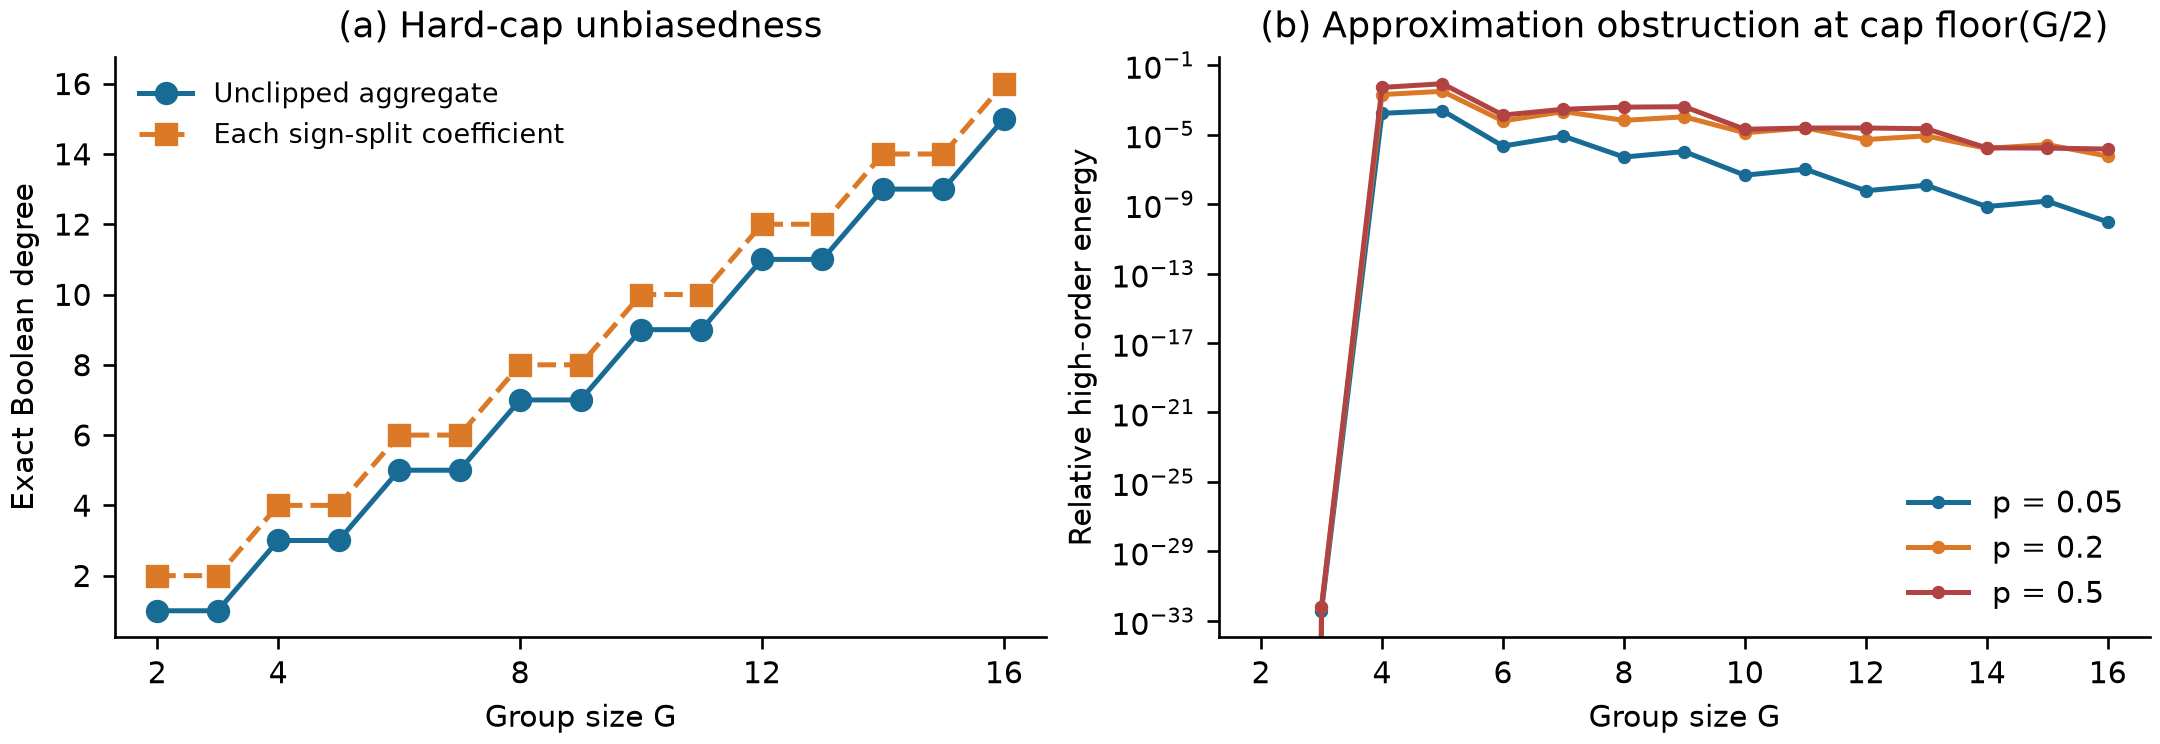
\includegraphics[width=\linewidth]{query_degree.png}
\caption{Exact query depth and its approximation limit. Left: the algebraic obstruction differs for the unclipped aggregate and sign-separated coefficients. Right: exact product-Bernoulli Fourier energy above a half-group hard cap, divided by the unclipped contrast's second moment. Small tail energy is a small integrated-bias lower bound; it is not a guarantee of a low-variance estimator.}\label{fig:degree}
\end{figure}

\section{Sequential completion under an expected budget}\label{sec:method}
Fix a label order $\pi$ using only pre-audit information. The completion maps are fixed independently of the stopping randomization $U$ and use only $X$ and the observed prefix. Let $\mu_k$ be any such computable completion vector after the first $k$ labels have been observed, with $\mu_G=\Phi(r)$. Choose absolute survival probabilities
\[
 1\ge Q_1\ge\cdots\ge Q_G\ge q_{\min}>0
\]
before querying. Draw $U\sim\operatorname{Uniform}(0,1)$, reveal the prefix for which $U<Q_k$, and return
\begin{equation}\label{eq:rr}
 \widehat\Phi=\mu_0+\sum_{k=1}^G\frac{\ind\{U<Q_k\}}{Q_k}(\mu_k-\mu_{k-1}).
\end{equation}
This is a finite randomized-telescoping estimator \citep{rhee2015,beatson2019}. We call its specified reward-audit instantiation sequential completion (SC).

\begin{theorem}[Conditional recovery of the complete-label surrogate]\label{thm:rr}
For every fixed complete label vector, any completion sequence with the correct endpoint, and any pre-audit positive survival schedule, $\E_I[\widehat\Phi\mid X,r]=\Phi(r)$. Consequently substituting $\widehat\Phi$ linearly into Equation~\eqref{eq:cliplinear} recovers $L_\theta(r)$ in expectation at each fixed $\theta$. If query costs are $c_{\pi_k}$, the expected incremental reference cost is $\sum_k Q_k c_{\pi_k}$.
\end{theorem}
\begin{proof}
Each indicator has conditional expectation $Q_k$. Taking expectations in the finite sum cancels the survival factors and telescopes to $\mu_G$. The objective and derivative conclusions follow by linearity. The cost is the sum of purchased query indicators times their fixed costs.
\end{proof}
A predictable adaptive order and continuation rule are also possible if each actual path probability is recorded correctly; the implementation and schedule optimization studied here use fixed pre-audit order and deterministic absolute survivals. This avoids confusing a fixed-chain optimum with an optimum over adaptive trees.

For clarity, an online implementation is the following. It receives a callback, not a vector of unqueried labels:
\begin{enumerate}
\item Freeze $p$, $\pi$, query costs and $Q$. Compute $\mu_0$ and draw one uniform $U$.
\item At step $k$, stop if $U\ge Q_k$. Otherwise buy label $r_{\pi_k}$ through the callback and compute the new completion $\mu_k$.
\item Add $(\mu_k-\mu_{k-1})/Q_k$ to the estimate. Return the estimate and the purchased indices.
\item Form the objective or update by a fixed linear map on the two coefficient blocks. Record purchased-query cost separately from prediction, scheduling and rollout computation.
\end{enumerate}
For zero stabilizer, each true advantage has magnitude at most $\sqrt{G-1}$. Conditional completions are bounded as well. A positive absolute survival floor therefore ensures finite second moments for this finite group, although the bound can be very loose and weights can still be large. Small successive continuation floors alone are less informative because their product can decay exponentially with depth.

\subsection{The strong whole-group baseline}
Let $I\sim\operatorname{Bernoulli}(q)$. The whole-group residual estimator
\begin{equation}\label{eq:whole}
 \widehat\Phi_{\mathrm{WG}}=\mu_0+\frac Iq\{\Phi(r)-\mu_0\}
\end{equation}
is already conditionally unbiased for the complete nonlinear vector. It corresponds to $Q_k=q$ for every $k$ and has expected cost $q\sum_i c_i$. Its conditional squared-error risk is
\[
 (q^{-1}-1)\norm{\Phi(r)-\mu_0}^2.
\]
It requires no intermediate completions. Comparing SC only with individual reward correction followed by normalization would omit this inexpensive and mathematically valid competitor.

\subsection{Independent-Bernoulli completion}\label{sec:completion}
Use an independent working model $R_i\sim\operatorname{Bernoulli}(p_i)$ and set $\mu_k=\E_p[\Phi(R)\mid R_{\pi_1},\ldots,R_{\pi_k}]$. The model is a variance-reduction device, not an assumption of Theorem~\ref{thm:rr}. Wrong marginal predictions and dependent actual labels do not change its endpoint; they can harm efficiency. To define completions even after a working-model zero-probability observation, observed coordinates are clamped to their actual labels and unobserved coordinates retain their original Bernoulli probabilities.

For $0<K<G$ define $a(K)=\sqrt{(G-K)/K}$ and $b(K)=-\sqrt{K/(G-K)}$, with both zero at $K=0,G$. Then $A_i^+=r_i a(K)$ and $A_i^-=(1-r_i)b(K)$. Poisson-binomial convolution computes the distribution of the unknown success count. Leaving out each unknown variable in turn gives the exact coordinate expectations. A straightforward implementation takes $O(G^3)$ work for one full vector, avoids sampling artificial labels, and handles already observed coordinates by replacing their probabilities with zero or one. Computing all $G$ prefix vectors thus takes $O(G^4)$ with this reference implementation. Exhaustive binary-cube checks validate the count calculation independently.

\subsection{A model-based schedule and its scope}\label{sec:schedule}
When the working model is correct, $\mu_k$ is a Doob martingale. Put $v_k=\E_p\norm{\mu_k-\mu_{k-1}}^2$. Orthogonality gives the model-averaged audit MSE
\begin{equation}\label{eq:modelrisk}
 \E_p\E_I\norm{\widehat\Phi-\Phi}^2=\sum_k v_k(Q_k^{-1}-1).
\end{equation}
The fixed-order optimization is therefore
\begin{equation}\label{eq:opt}
 \min_Q\sum_k v_k/Q_k,\quad
 \sum_k c_{\pi_k}Q_k\le B,\quad
 1\ge Q_1\ge\cdots\ge Q_G\ge q_{\min}.
\end{equation}
A weighted pool-adjacent-violators calculation merges neighboring blocks when their ratios $\sum v/\sum c$ violate nonincrease. For a block $\mathcal B$, its common survival is
\begin{equation}\label{eq:pava}
 Q_{\mathcal B}=\clip\left(
 \sqrt{\frac{\sum_{k\in\mathcal B}v_k}{\lambda\sum_{k\in\mathcal B}c_{\pi_k}}},q_{\min},1\right),
\end{equation}
with $\lambda$ chosen to satisfy the budget when it is active. Zero-variance tails can leave legitimate slack; positive survival is retained for robustness to a wrong model. Appendix~\ref{app:moments} gives an exact $O(G^4)$ count-compressed formula for the $v_k$, so this schedule needs no additional true labels for calibration.

This optimality claim is deliberately narrow: independent working model, fixed order, deterministic survival, specified costs, and Euclidean coefficient MSE. It is not a guarantee for misspecified labels, arbitrary policy-gradient geometry, or adaptive query trees. Scheduling has a measurable computational cost. In a homogeneous completion model it can reduce to Equation~\eqref{eq:whole}, an outcome to report rather than conceal.

\section{Empirical study}\label{sec:experiments}
We separate algebraic verification, controlled estimation, constructed policy training, and historical software-trajectory diagnostics. Each level has a different estimand. Local design records were written before the corresponding run; later extensions are identified as such. They were not registered with an external preregistration service. No paid cloud resources, fresh software-agent rollouts, or large-model reinforcement-learning runs are represented by the results below.

\subsection{Exact checks and controlled fixed groups}\label{sec:controlled}
Independent checks enumerate the degree formula for $G=2,\ldots,12$, integrate all stopping paths for fixed binary groups, verify the sign-split clipping identity and its derivative, and compare the schedule solver with constrained numerical optimization. The M\"obius coefficient formula agrees to $2.21\times10^{-14}$. Exact adaptive stopping checks agree to $5.56\times10^{-17}$. A separate implementation enumerates all $65{,}536$ label configurations at $G=16$ to verify the count-compressed model moments; the largest discrepancy is $4.45\times10^{-14}$. These are arithmetic validation results, not training-performance measurements.

The initial controlled study uses $G\in\{4,8,16\}$, logistic-normal base-rate parameter $\alpha\in\{.05,.2,.5,.8,.95\}$, and three completion regimes. Draw $z_i\sim N(\operatorname{logit}\alpha,1.2^2)$ and supply $p_i=\operatorname{sigmoid}(z_i)$. True labels are independent Bernoulli with probabilities $p_i$, $\operatorname{sigmoid}(.45z_i)$, or $\operatorname{sigmoid}(-.65z_i)$ for calibrated, overconfident and shifted cases. The input $\alpha$ is not the achieved marginal success rate. Costs are normalized lognormal draws in simulated units. A fixed random six-dimensional linear map with clipping masks supplies a gradient-like projection; it is not a language-model gradient.

For each of 45 group-size/base-rate/regime combinations, 64 separate development groups choose a survival exponent from $\{0,.5,1,2\}$. There are 256 evaluation groups and budget fractions $\{.25,.5,.75\}$, making 135 setting-budget comparisons. All methods share each evaluation group. Prefix estimators and whole-group correction are integrated exactly over all stopping depths. Individual reward correction and partial replacement enumerate all audit masks for $G=4,8$ and use 1,024 masks for $G=16$. The latter squared-bias estimates receive a signed finite-Monte-Carlo correction, detailed in Appendix~\ref{app:protocol}; negative corrected values are retained.

\paragraph{Calibration cost changes the result.}
At the same marginal audit budget, the development-tuned sequential estimator has mean projected-MSE ratio $0.9015$ and median $0.9713$ relative to whole-group correction across the 135 comparisons. The mean ratios by regime are $0.7442$, $0.9595$ and $1.0008$. However, the 64 complete development groups cost another $64G$ labels. Amortizing this cost over 256 evaluation groups allows the baseline to use $q'=\min(1,q+.25)$. The tuned method improves on this cost-matched baseline in \emph{zero of 135} comparisons. The development labels are shared across the three evaluated budgets; they must neither be charged three times nor omitted. This negative result motivated the subsequent model-based schedule of Section~\ref{sec:schedule}.

\begin{figure}[t]
\centering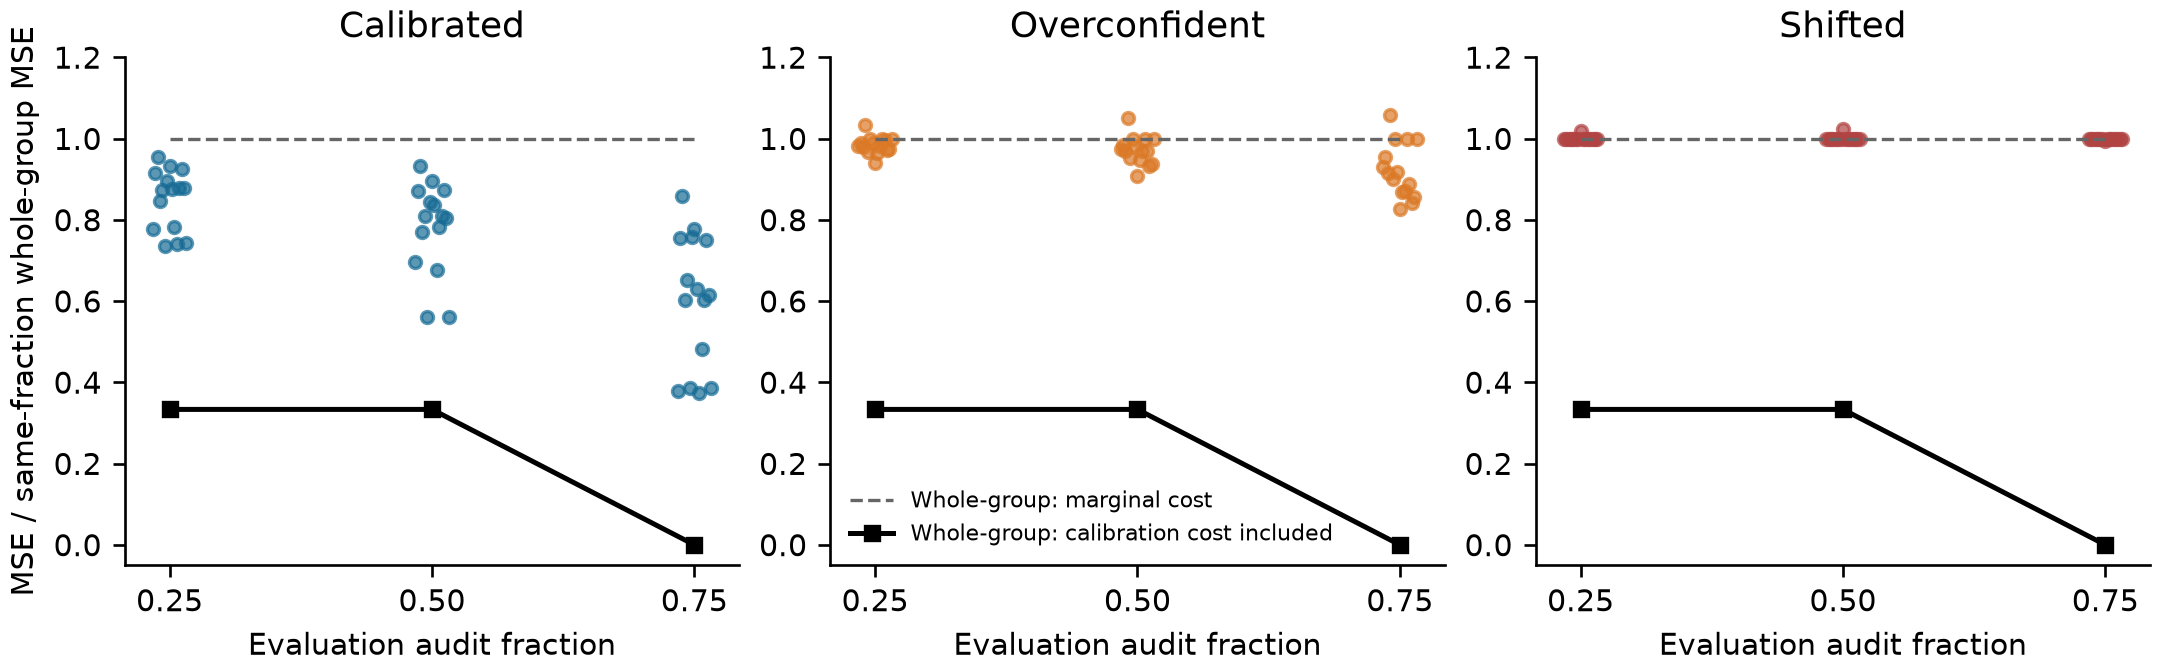
\includegraphics[width=\linewidth]{calibration_cost.png}
\caption{Initial study: each colored point is a tuned sequential setting's projected-MSE ratio to whole-group correction at the same marginal audit fraction. The black line gives whole-group MSE when allowed the same total label expenditure, including the sequential method's 64-group development cost amortized across 256 evaluation groups. At fraction .75 the comparator can afford full labels and its audit MSE is zero.}\label{fig:calibration}
\end{figure}

\subsection{A subsequent model-only scheduling experiment}
After the calibration-cost finding, we froze a label-free alternative using the model moments and PAVA rule, and evaluated it with fresh seed 20260914. The same grid has 135 budget settings, each with 256 groups; all methods share each group and its supplied predictor. No reference labels fit the predictor or tune this schedule. We exactly integrate stopping-depth randomness and retain every setting. The base-rate grid specifies the logistic-normal intercept, not the realized success prevalence.

\begin{table}[t]
\centering
\caption{Subsequent model-only schedule versus whole-group residual correction at the same expected label-cost ceiling. Ratios are medians across 45 settings per regime; wins count lower group-averaged MSE. The fixed six-dimensional map is a synthetic linear-update diagnostic.}
\label{tab:model-only}
\begin{tabular}{lrrrr}
\toprule
&\multicolumn{2}{c}{Coefficient MSE}&\multicolumn{2}{c}{Six-dimensional MSE}\\
Regime&Ratio&Wins&Ratio&Wins\\
\midrule
Calibrated&0.748&45/45&0.726&45/45\\
Overconfident&1.021&18/45&0.984&26/45\\
Shifted&2.243&0/45&1.898&0/45\\
\bottomrule
\end{tabular}
\end{table}

Correct-model gains coexist with substantial misspecification losses (Table~\ref{tab:model-only}); the worst shifted coefficient ratio is 6.68. The largest conditional coefficient-bias square is $2.94\times10^{-30}$, so this failure is variance rather than failed correction. Model optimality concerns coefficient risk under the supplied model and a fixed order, not the projected update or an incorrect model. Computation also increases: for $G=16$, mean scheduling CPU is 5.24\,ms and scheduling plus expected completion CPU is 10.38\,ms, versus 0.55\,ms for whole-group correction. These Python microbenchmarks exclude actual verifier execution and do not imply a training speedup. Raw groups, schedules, paired standard errors, all costs, and independent full-cube checks accompany the release.

\begin{figure}[t]
\centering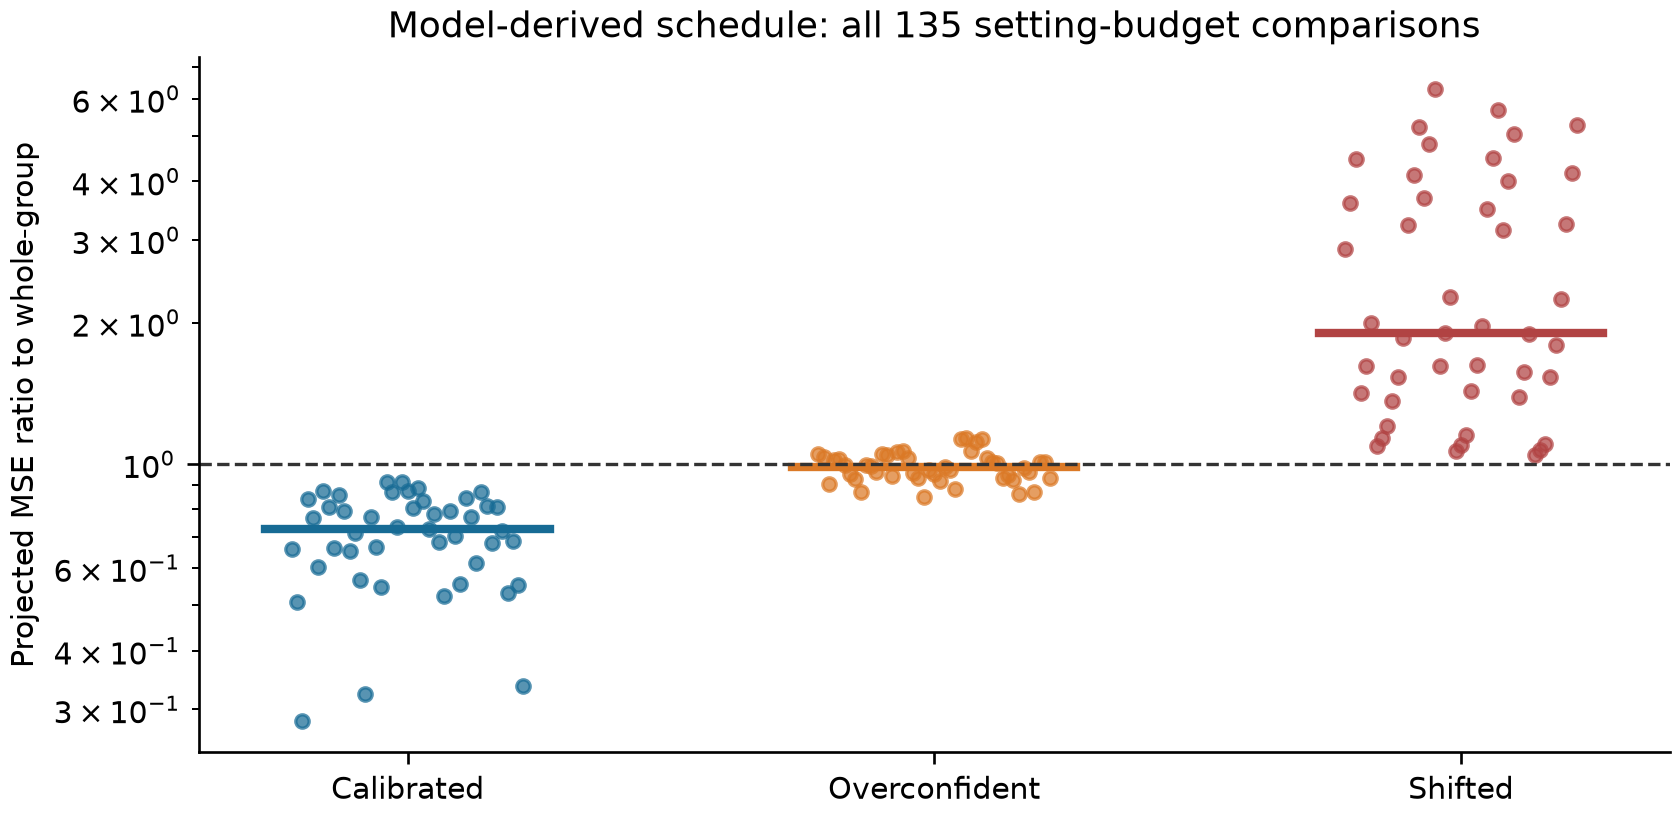
\includegraphics[width=.85\linewidth]{model_schedule.png}
\caption{New-seed model-derived schedules: all 45 setting-budget points per regime. Each point is a 256-group mean projected-MSE ratio to whole-group residual correction; bars are descriptive medians. The three budgets share groups. A correct working model helps, while reversed label probabilities can substantially increase variance despite retained conditional unbiasedness.}\label{fig:model}
\end{figure}

% Requires booktabs. Detailed protocol: stateful_appendix.tex.
\subsection{Controlled training with stateful dependency tools}
\label{sec:stateful-training}

We test whether the label estimators support actual policy updates in a
constructed release-repair environment. A component build records the current
artifact of its parent; changing an upstream component can therefore leave
downstream builds, attestations, and published artifacts stale. The cheap
checker inspects only published local versions, whereas the reference checker
executes all dependency and provenance constraints. These are deterministic
tools and a NumPy softmax policy, not a language model or a public software
benchmark.

We run all six methods for 300 on-policy updates, with groups of eight
trajectories, horizons $H\in\{12,24,48\}$, and ten independent training seeds
per setting. All methods infer reference failure for free when the necessary
cheap check fails. If $M$ candidate labels remain, each partial method purchases
$M/2$ labels in expectation. The completion probabilities and sequential
survival schedule are fixed before training. Evaluation uses 256 independent
reporting episodes per checkpoint, paired across methods within a seed.

\begin{table}[t]
\centering
\small
\setlength{\tabcolsep}{4pt}
\begin{tabular}{lrrr}
\toprule
Method & $H=12$ & $H=24$ & $H=48$ \\
\midrule
Full-label update & $94.06\pm0.61$ & $83.44\pm1.03$ & $57.97\pm0.96$ \\
Cheap labels only & $17.42\pm3.58$ & $19.84\pm2.92$ & $3.59\pm0.95$ \\
Whole-group residual & $93.48\pm0.71$ & $83.24\pm1.05$ & $55.27\pm1.16$ \\
Sequential completion & $93.55\pm0.63$ & $83.05\pm0.88$ & $56.60\pm1.72$ \\
Reward HT then normalize & $86.84\pm0.47$ & $68.91\pm1.07$ & $32.23\pm1.24$ \\
Partial replacement & $91.13\pm0.58$ & $75.08\pm0.68$ & $29.96\pm1.76$ \\
\bottomrule
\end{tabular}
\caption{Reference-check success (\%, mean $\pm$ standard error across ten
training seeds) after the same 2,400 training trajectories per run.
Purchased-label counts differ. The initial mean success rates were
$40.08\%$, $18.55\%$, and $4.96\%$, respectively.}
\label{tab:stateful-training}
\end{table}

Sequential completion (SC) and the strong whole-group residual baseline reach similar
mean endpoints (Table~\ref{tab:stateful-training}); all three paired,
pointwise 95\% intervals for their difference include zero. Thus these runs do
not establish a distinct benefit from the fixed sequential schedule. Nor does
an interval containing zero establish equivalence to full-label training.
Cheap-label optimization can instead improve the incomplete checker while
retaining poor reference success: at $H=48$, its endpoint cheap success is
$92.38\%$, versus $3.59\%$ under the reference checker.

Across the 30 runs for each method, SC purchases 30,908 training labels,
compared with 62,508 for full-label updates and 30,832 for whole-group residual
correction. This query reduction is not a measured speedup: training takes
29.08, 19.79, and 21.35 seconds, respectively, with these inexpensive checks.
The scripted initialization already executes the known workflow greedily;
this experiment measures stochastic execution reliability, not discovery of
an unknown repair procedure. Further protocol, accounting, and inferential
limits appear in Appendix~\ref{app:stateful-training}.

\begin{figure}[t]
\centering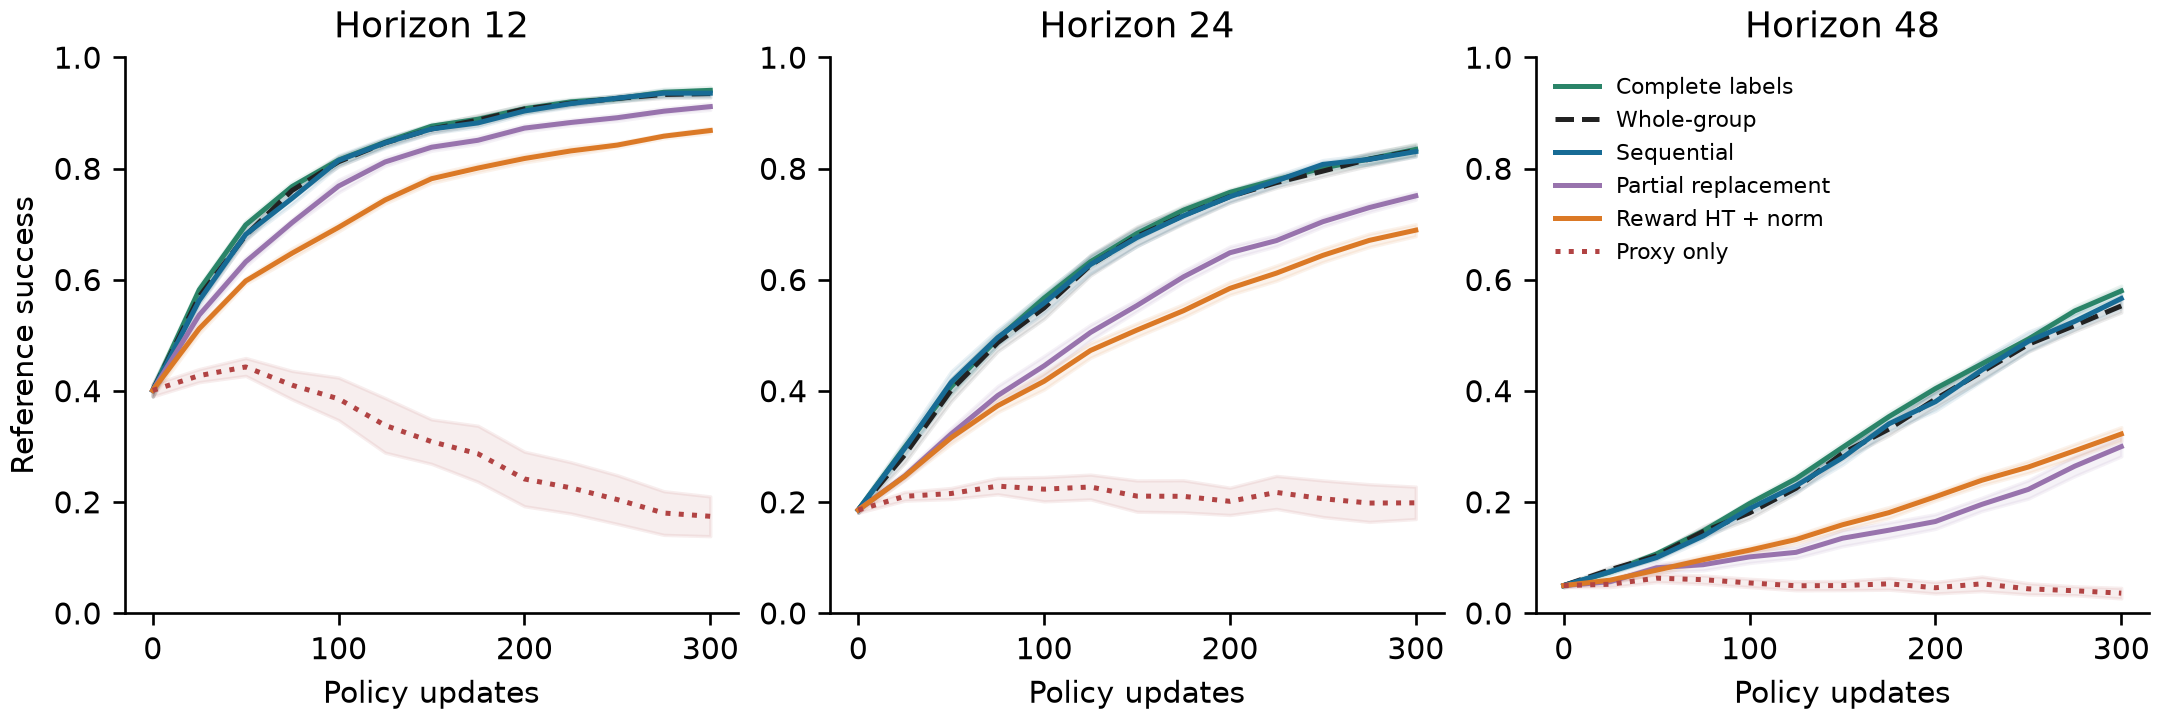
\includegraphics[width=\linewidth]{stateful_training.png}
\caption{Constructed stateful policy training. Lines average ten training seeds; bands show one pointwise seed standard error. Every method uses the same number of rollout groups. Proxy-only training can improve the cheap criterion while losing reference success. The sequential and whole-group curves do not establish a difference between those methods.}\label{fig:training}
\end{figure}

\subsection{Historical software records and frozen-model geometry}\label{sec:frozen}
We use the official SWE-Gym historical trajectory release \citep{pan2025,swegymdata}. Strict groups sharing both task and logging configuration have size at most two, so no strict G8 group is available. A recorded availability amendment forms fixed heterogeneous same-task groups; the heldout G8 set has 49 tasks, 392 records and 22 mixed-label groups. All 49 groups are retained. This is historical empirical replay, not on-policy data collection or a new SWE-bench evaluation.

A frozen Qwen2.5-Coder-1.5B-Instruct checkpoint supplies a specified 32-dimensional added-logit-bias score \citep{qwenmodel}. Inputs preserve tool call arguments but score only a bounded-context final assistant body. Independent autograd, finite-difference and token-mask checks validate the extraction definition. The evaluation target is the complete-label empirical surrogate in this parameter subspace. It makes no claim about full-parameter gradients or training improvement. Appendix~\ref{app:historical}--\ref{app:frozen} gives the group, split, proxy, serialization and parameterization details.

\begin{table}[t]
\centering\small
\begin{tabular}{lrrr}
\toprule
Method & $q=.25$ & $q=.50$ & $q=.75$\\
\midrule
Complete labels & 0.000 & 0.000 & 0.000 \\
Whole-group residual & 1.000 & 1.000 & 1.000 \\
Fixed sequential & 1.488 & 1.352 & 1.027 \\
Model coefficient schedule & 0.831 & 0.759 & 0.683 \\
Model gradient schedule & 0.896 & 0.861 & 0.744 \\
Reward HT then normalize & 0.770 & 1.937 & 4.861 \\
Partial replacement & 0.772 & 1.965 & 4.479 \\
Proxy completion & 0.333 & 1.000 & 3.000 \\
\bottomrule
\end{tabular}
\caption{Historical frozen-score diagnostic: ratio of mean 32-dimensional empirical gradient MSE to whole-group residual correction. Every row includes the same 49 tasks. Values below one favor the row; full verification uses eight labels and proxy completion uses zero, so these two rows have different costs. Other rows use expected label counts 2, 4 and 6. Biased estimators may have lower MSE.}\label{tab:frozen}
\end{table}

Model coefficient schedules reduce mean projected MSE relative to whole-group correction by $16.9\%$, $24.1\%$ and $31.7\%$ at the three audit fractions (Table~\ref{tab:frozen}). Their paired task-bootstrap ratio intervals are $[.684,.992]$, $[.547,.996]$ and $[.348,1.119]$. These are pointwise descriptive intervals over 49 historical tasks; they are not simultaneous claims across budgets. The fixed exponent-one schedule instead loses to whole-group correction at each fraction. The gradient-model schedule also has lower mean error than whole-group correction, but performs worse than the coefficient-model schedule here and its intervals include one. This does not contradict model optimality: the frozen independent label model need not match the empirical conditional label/score relationship.

The full extraction evaluates 57,948 target tokens. Forward and score computation take 763.20 seconds; the invocation including model setup takes 778.82 seconds on the shared M1 Pro host. The audit-risk calculation then exactly integrates the stopping paths or independent masks; it does not execute tests or train a policy. Proxy completion has the lowest MSE among several methods at the smallest budget despite nonzero conditional bias. Thus design unbiasedness is a target-preservation property, not by itself a minimum-MSE or learning-quality guarantee.


\section{Related work}\label{sec:related}
Importance-weighted estimation has a long history \citep{horvitz1952}. Active statistical inference combines predictions with selectively acquired labels \citep{zrnic2024}; robust sampling explicitly addresses failures of an estimated uncertainty allocation \citep{li2025}. Doubly robust reinforcement-learning estimation and policy-gradient constructions are also established \citep{jiang2016,huang2020}. Our audit inclusion probability is distinct from a policy's action probability, and we do not infer off-policy validity from correct audit weights.

Randomized telescoping and unbiased random truncation are the direct foundations of Equation~\eqref{eq:rr} \citep{rhee2015,beatson2019}. The fixed-chain cost--variance optimization is an application of that design principle. Multi-fidelity policy gradients already combine accurate and approximate information using control variates and address both reward and dynamics differences \citep{liu2026}. We condition on fixed trajectories and correct only missing reference labels. A cheap environment that changes states or observations changes the trajectory distribution, which this correction cannot repair.

Recent verifier-noise corrections already recognize that reward calibration and group normalization interact. In version~4, \citet{cai2025} explicitly shows that current-group standardization can cancel binary affine corrections, and implements direct trajectory coefficients with leave-one-out baselines and fixed or running scales. Its selective appeals mechanism uses Horvitz--Thompson counts to estimate false-negative rates, so budgeted verification within policy training is also established. The stated gradient guarantees concern an oracle class-conditional channel before finite-group normalization and clipping; the implementation additionally discusses instance-dependent residual bias and audits the advantages actually passed to training.

Version~3 of \citet{mansouri2025} likewise identifies affine invariance and corrects both reward moments and normalization. Its exact GRPO comparison requires the oracle population standard deviation; the practical corrected-variance normalizer is a consistent plug-in approximation. The paper also includes an empirical clipping ablation. These distinctions prevent interpreting our elementary counterexamples as refutations of either paper's analyzed variants.

Our estimand is the normalized or clipped update of one fixed, completely labelled finite group. We randomize reference-label queries and seek exactness conditional on that group's trajectories and potential labels, without identifying a reward-flip channel. This preserves a specified nonlinear surrogate; it does not establish that preserving that surrogate is preferable to using the simpler alternative objectives studied in prior work.


The polynomial representation of query algorithms is classical; query complexity in expectation studies related polynomial characterizations under different output restrictions \citep{kaniewski2015}. We permit signed outputs and give the elementary decision-tree argument directly. The specialized result is the exact degree of the group-normalized binary function. GRPO and PPO provide the training objectives being analyzed \citep{shao2024,schulman2017}. SWE-Gym supplies real software-agent trajectories for a separate historical diagnostic \citep{pan2025}; using its records does not constitute rerunning its benchmark or reproducing its training results.

\section{Limitations and implications}
Pointwise unbiasedness protects a specified complete-label objective, not necessarily the objective best aligned with downstream task success. Low-variance biased methods can be preferable under limited computation. The approximation spectrum and the strong whole-group baseline both make this limitation concrete. Moreover, clipping gradients, applying Adam, choosing checkpoints on the same audit sample, or reusing an audited batch adaptively does not preserve equality of optimizer trajectories. The theorem should be applied to a freshly specified fixed-parameter update; practical multiple-epoch reuse needs its own analysis.

The independent-Bernoulli completion model ignores within-task label dependence. Its predictive accuracy, calibration and score-weighted residuals can shift during training. Positive audit probabilities retain conditional unbiasedness, but large corrections can destabilize optimization. Query costs were simulated in the controlled study and are extremely cheap in the constructed environment. Historical verdict replay measures label acquisition counts, not elapsed time for executing a real test suite. None of these studies establishes an end-to-end software-agent training speedup.

The constructed tasks train stochastic execution reliability from a scripted initial policy; they do not demonstrate planning discovery or generalization to unseen repositories. The historical model diagnostic evaluates a declared truncated empirical target in a small added parameter subspace, not a full-parameter on-policy gradient. Scaling to fresh language-model training requires executable sandboxed tasks, measured verifier latency, strong whole-group correction, and multiple independent training seeds with rollout, verifier and scheduler costs all accounted for.

A useful practical rule follows from the analysis: decide which nonlinear update must be estimated before choosing an audit unit. Whole-group residual correction is a valid low-complexity starting point. A sequential design earns its extra complexity only when its reduction in the relevant error outweighs intermediate-completion, scheduling and calibration costs.

\section*{Reproducibility statement}
The accompanying source contains the online query callback, independent algebraic checks, complete controlled group arrays, constructed-environment action and audit ledgers, frozen executed-source snapshots, public-source manifests, and scripts that generate the reported tables. Appendix~\ref{app:protocol} identifies seeds, computational scope and post-run reporting corrections. The private direction notes, model weights and raw third-party trajectory text are not included in the release package. Public inputs are referenced by pinned revisions and checksums.

\section*{AI assistance statement}
AI assistance was used extensively for literature discovery, mathematical derivation, manuscript preparation, code implementation and computational checks. Numerical results reported here come from executed programs and saved artifacts. Independent implementations and programmatic checks were used to test core claims; these checks do not replace expert review or establish originality. This statement describes the preparation process and does not certify a separate human verification process that has not been recorded.

\section*{Data and research scope}
The research uses constructed tasks and publicly released historical software-agent records. No new human-subject study or internal corporate dataset is involved. Reference success denotes the specified test or invariant verdict, not proof of all intended program behavior. The public trajectory card did not provide an explicit dataset license at retrieval; the package supplies provenance and retrieval instructions rather than redistributing those raw records.

\bibliographystyle{plainnat}
\bibliography{references}
\clearpage
\appendix
\section{Proof of the exact degree theorem}\label{app:proof}
Let $c_i=s_i-G^{-1}\sum_j s_j$, so $\sum_i c_i=0$. If $0<K<G$, substitution into Equation~\eqref{eq:F} gives
\[
 F_s(r)=\frac{\sum_i c_i r_i}{\sqrt{K(G-K)}}.
\]
Both constant-label endpoints are zero. A Boolean function has a unique multilinear representation $F_s(r)=\sum_S a_S\prod_{i\in S}r_i$. For a proper subset $S$ of size $\ell$, M\"obius inversion yields
\begin{align*}
 a_S&=\sum_{T\subseteq S}(-1)^{\ell-|T|}F_s(\ind_T)\\
 &=\sum_{j=1}^{\ell}(-1)^{\ell-j}f(j)
       \sum_{\substack{T\subseteq S\\|T|=j}}\sum_{i\in T}c_i\\
 &=\left(\sum_{i\in S}c_i\right)
       \sum_{j=1}^{\ell}(-1)^{\ell-j}\binom{\ell-1}{j-1}f(j)
 =\left(\sum_{i\in S}c_i\right)\Delta^{\ell-1}f(1).
\end{align*}
The full-set coefficient is zero. For every $j=1,\ldots,G-1$, the sum over all size-$j$ subsets is $\binom{G-1}{j-1}\sum_i c_i=0$, and both endpoints contribute zero.

To control the sign of the remaining differences, set $a=G/2$ and $z=x-a$. For $0<x<G$,
\[
 f(x)=\frac1a\left(1-\frac{z^2}{a^2}\right)^{-1/2}
 =\frac1a\sum_{n=0}^{\infty}\frac{\binom{2n}{n}}{4^n}
   \frac{z^{2n}}{a^{2n}}.
\]
This power series can be differentiated termwise on compact subintervals. Every even derivative is strictly positive: every surviving term is nonnegative, and the term $n=j$ in derivative order $2j$ is a positive constant. Iterating the fundamental theorem of calculus gives
\[
 \Delta^m f(x)=\int_{[0,1]^m} f^{(m)}(x+t_1+\cdots+t_m)\,dt_1\cdots dt_m,
\]
whenever the interval lies inside $(0,G)$. Hence every even-order difference used above is strictly positive.

If $G$ is even, set $\ell=G-1$. The difference order is $G-2$, even and positive. Since $c$ is nonzero, omit an index with $c_i\ne0$; the sum of $c$ over the remaining indices is $-c_i\ne0$. Thus there is a nonzero coefficient of degree $G-1$, and none of degree $G$.

If $G$ is odd, the difference of order $G-2$ on $f(1),\ldots,f(G-1)$ vanishes: the points pair about $G/2$, $f(j)=f(G-j)$, and paired binomial coefficients have opposite signs. All degree-$G-1$ coefficients vanish. For $\ell=G-2$, the difference has the positive even order $G-3$. If every subset of this size had zero $c$ sum, the complementary pairs would all obey $c_i+c_j=0$. For $G\ge3$, this forces all $c_i=0$, a contradiction. Therefore a nonzero degree-$G-2$ coefficient exists.

For the query implication, fix the internal random seed of any adaptive algorithm. Its leaf event is a product of literals $r_i$ or $1-r_i$ along a path. Repeated queries of a deterministic label reveal nothing new, so a hard cap $b$ bounds the degree of each leaf-event polynomial by $b$. Multiplying by the output at that leaf and summing still gives degree at most $b$. Integrability and the finite cube permit expectation over internal seeds, leaving the mean function in the same finite-dimensional space. It cannot equal $F_s$ when $b<d_G$.

For the existence statement, sample a nonzero monomial $S$ with any positive probability $p_S$, query its variables, and output $a_S\prod_{i\in S}r_i/p_S$. Include a constant term if present. A finite number of bounded outputs gives finite variance. This establishes attainability of the query cap, without establishing practical variance or computational efficiency of the monomial representation.

\section{Variance identities and model moments}\label{app:moments}
\subsection{Conditional variance under a fixed label vector}
Write $D_k=\mu_k-\mu_{k-1}$ and $I_k=\ind\{U<Q_k\}$. For $j<k$, nested inclusion gives $\E[I_jI_k]=Q_k$. Thus
\[
 \operatorname{Cov}(I_j/Q_j,I_k/Q_k)=Q_j^{-1}-1.
\]
Consequently the conditional Euclidean MSE is
\begin{equation}\label{eq:conditionalrisk}
 \E_I\norm{\widehat\Phi-\Phi}^2
 =\sum_k(Q_k^{-1}-1)\norm{D_k}^2
 +2\sum_{j<k}(Q_j^{-1}-1)\langle D_j,D_k\rangle.
\end{equation}
The cross terms generally do not vanish for a fixed true label vector. Replacing this expression with $\sum_k\norm{D_k}^2(1/Q_k-1)$ on every observed group is incorrect. Orthogonality holds after averaging under the correct conditional-completion model. In that case $\E_p[D_k\mid\mathcal H_{k-1}]=0$, so $\E_p\langle D_j,D_k\rangle=0$ for $j<k$, proving Equation~\eqref{eq:modelrisk}. With a fixed linear target map $L$, replace the norm by $\norm{L^\top D_k}$; the optimal schedule can differ from one minimizing coefficient MSE.

\subsection{Count-compressed second moments}
Relabel coordinates in their query order. Let $S_k=\sum_{i\le k}R_i$, $U=\{k+1,\ldots,G\}$, and $K_U=\sum_{i\in U}R_i$. Define
\begin{align*}
 a_s&=\E_p[a(s+K_U)], & b_s&=\E_p[b(s+K_U)],\\
 \alpha_i(s)&=p_i\E_p[a(s+1+K_{U\setminus\{i\}})],&
 \beta_i(s)&=(1-p_i)\E_p[b(s+K_{U\setminus\{i\}})].
\end{align*}
Here $a,b$ have the endpoint convention given in Section~\ref{sec:completion}.
\begin{lemma}[Exact completion moments]\label{lem:moments}
For the independent-Bernoulli working model,
\begin{equation}\label{eq:moment}
 M_k:=\E_p\norm{\mu_k}^2
 =\sum_{s=0}^{k}\Pr_p(S_k=s)\left[
 s a_s^2+(k-s)b_s^2+
 \sum_{i\in U}\{\alpha_i(s)^2+\beta_i(s)^2\}\right].
\end{equation}
Moreover $v_k=M_k-M_{k-1}\ge0$,
\[
 M_0=\norm{\E_p\Phi}^2,\qquad
 M_G=G\left[1-\prod_i p_i-\prod_i(1-p_i)\right].
\]
\end{lemma}
\begin{proof}
Given an observed prefix with $s$ successes, each known positive coordinate has conditional coefficient $a_s$ and each known negative coordinate has coefficient $b_s$. Every unknown coordinate contributes the two conditional coefficients $\alpha_i(s),\beta_i(s)$. The Euclidean squared norm depends on the known prefix only through $s$, even if its individual probabilities differ. Averaging over its Poisson-binomial count gives Equation~\eqref{eq:moment}. The difference of moments is the squared martingale increment by the conditional-expectation projection identity. Finally, every mixed binary group has $\sum_i A_i^2=G$, while an all-equal group has zero norm. The probabilities of the two all-equal groups give the endpoint formula.
\end{proof}
The implementation caches prefix, suffix and leave-one-out count distributions before the sum over $s$. Constructing these distributions inside every term would introduce unnecessary work. The reference calculation takes $O(G^4)$ overall, using polynomial convolution and finite sums. A general gradient-weighted norm can depend on which prefix coordinates succeeded, so the same count-only formula cannot be asserted for an arbitrary weight matrix.

\subsection{Monotone survival optimization}
Ignoring the constant $-\sum_kv_k$, Equation~\eqref{eq:modelrisk} gives a separable convex objective. For a Lagrange multiplier $\lambda\ge0$ and a block on which the monotone constraint is active, its first-order equation is
\[
 -\frac{\sum_{k\in\mathcal B}v_k}{Q_{\mathcal B}^2}
 +\lambda\sum_{k\in\mathcal B}c_{\pi_k}=0.
\]
The block solution is Equation~\eqref{eq:pava}. Adjacent blocks whose $\sum v/\sum c$ ratios increase must be pooled; the resulting nonincreasing blocks satisfy the monotone KKT conditions. Common lower and upper bounds clip those block solutions. A scalar search chooses the multiplier. If all $v_k=0$, every feasible positive schedule minimizes the modeled risk, and we use uniform survival. With only a zero-variance tail, its floor may permit a slack budget after every useful block has reached one. Actual expected cost is always calculated as $Q^\top c$, not copied from the requested budget.

The solver normalizes a nonzero variance vector by its maximum before computing the shape. An absolute threshold such as ``sum of variances below $10^{-15}$ means zero'' would break scale invariance and can return a wrong uniform schedule for a small but informative gradient. An independent test exposed this issue before the subsequent model-scheduled study; its correction and the original source snapshot are retained.

\section{Additional counterexamples and implementation boundaries}
\paragraph{Post-audit fitting can invalidate augmentation.}
For a single true label $r=1$, audit probability $q=1/2$, and a prediction set after observing the audit to $m=I$, Equation~\eqref{eq:ht} returns $I$ and has expectation $1/2$. The claim that predictions can be wrong is not permission to refit them on the same unaccounted audit outcome. Freeze predictions, train on past data, or use an appropriate independently specified cross-fitting scheme.

\paragraph{Reference-label correction does not correct dynamics.}
Suppose the full environment begins in state $s_1$ while a cheap simulator begins in state $s_0$, and the policy has independent parameters for the two states. Reward correction on the cheap trajectory can never create the missing score coordinate at $s_1$. Its update still targets the wrong occupancy distribution. A trajectory-level multi-fidelity method or a separate dynamics analysis is necessary \citep{liu2026}.

\paragraph{Adaptive selection of parameters changes conditioning.}
For every fixed $\theta$, Equation~\eqref{eq:rr} defines an unbiased random surrogate. Selecting $\theta$ by optimizing that same random function makes $\theta$ dependent on its noise. The pointwise expectation cannot be substituted at that random optimum. Similarly, norm clipping, Adam preconditioning and checkpoint selection are nonlinear. The constructed experiment records whether gradient clipping activates; it does not claim that its optimizer path equals complete-label training.

\paragraph{Hard-cap degree and the label domain.}
The query-degree theorem assumes every binary vector remains feasible after conditioning on the declared cheap information. If a cheap negative is a proven negative of the stronger test, that coordinate is already known. A learned classifier's high average accuracy is not such a logical certificate. The construction in Appendix~\ref{app:stateful} uses an exact implication and gives its benefit to the complete-verification and whole-group baselines as well as SC.

\section{Constructed stateful training: protocol and accounting}
\label{app:stateful-training}
\label{app:stateful}

\paragraph{Environment.}
There are $n=H/4$ components in a directed dependency chain. Initially their
source, cached artifacts, attestations, and publications all reflect version
zero. The task changes the required version of one component, sampled
uniformly from the first $\lceil n/2\rceil$ positions, to one. Each component is
visited once in each of four rounds, in topological order. Every visit permits
one of five actions: no operation, edit source to the specification, build,
attest, or publish. These are actual tool-state transitions, including legal
no-ops. A build stores the current built parent prefix followed by the local
source version; attestations and publications retain immutable fingerprints.
Consequently, updating an upstream component does not automatically refresh
its dependants.

The reference verifier executes four constraints per component: the source
matches its requested version, and the artifact, attestation, and publication
each match the required complete prefix. The cheap verifier checks only the
local version of each published artifact. Its failures are conclusive
reference failures; every baseline uses this common shortcut. The observation
contains 15 features: an intercept, four phase indicators, local source and
requested versions, five inspectable metadata comparisons, and normalized
position, remaining horizon, and problem size. Constructing this observation
does not invoke the reference verifier. Public task requirements are not
hidden supervision; the purchased terminal labels are isolated from action
selection and unqueried estimator inputs.

\paragraph{Policy and optimization.}
A shared linear softmax maps these features to five action probabilities.
All methods initialize with probability $0.9$ on the round-appropriate action
and $0.025$ on each other action. This scripted prior is disclosed because a
nearly uniform policy would yield little terminal success at larger $H$.
The initial greedy policy already follows a correct workflow. We execute
300 updates per run, with eight newly sampled trajectories per update and
a learning rate of $0.5$. For trajectory $i$, the score is the mean action
score, $H^{-1}\sum_{t=1}^{H}\nabla_\theta\log\pi_\theta(a_{it}\mid o_{it})$.
The estimated group coefficients weight these scores in one on-policy SGD
update. There are no Adam updates, replay epochs, learned critics, or auxiliary
rewards. The norm cap is one; it activates in none of the 54,000 updates
(maximum observed norm $0.642$). Positive and negative coefficients are added
at likelihood ratio one, so these runs do not test off-policy clipping.

\paragraph{Auditing rules.}
After cheap-negative certification, $M$ candidate labels remain in their
original order. The completion model assigns them probability $0.55$ and
assigns certified negatives probability zero. It is fixed and not fitted on
training or reporting labels. Whole-group residual correction buys all $M$
labels with probability $1/2$ and otherwise uses the same completion vector.
Sequential completion (\texttt{rr\_completion} in the released code) uses
\[
 Q_j=\operatorname{clip}\bigl(c j^{-1/2},0.005,1\bigr),
 \qquad \sum_{j=1}^{M}Q_j=M/2,
\]
with the scale $c$ chosen before observing any purchased label. The empty
candidate set needs no purchases. Reward HT independently buys candidates
with probability $1/2$, substitutes twice the observed reward and zero for
unbought candidates, and then normalizes. Partial replacement uses the same
inclusion probabilities but retains unbought cheap labels. Both are distinct
from correction of the final group coefficients.

A subsequent outcome-free diagnostic evaluated the model-based increment
second moments of the homogeneous completion prior. For every
$M\in\{1,\ldots,8\}$, the monotone schedule minimizing the model's Euclidean
coefficient error was $Q_j=1/2$ for every candidate. It therefore coincided
with whole-group residual correction. This is a boundary case of the
allocation problem, not a reason to replace the frozen primary schedule or
a claim about the true policy-gradient error.

\paragraph{Randomness and evaluation.}
Ten independent training seeds are used for each horizon and method. Within
a seed, task and action uniforms are paired across methods; learned policies
can still produce different subsequent trajectories. Audit randomness uses a
separate stream. Reporting uses 256 stochastic episodes at update zero and
every 25 updates, with a separate stream reused for pairing across checkpoints
and methods. Reporting labels do not select parameters, schedules, updates, or
stopping rules. These are independent episode draws from the declared task
family, not unseen repository tasks. The horizon and chain size co-vary, so
their individual effects are not identified.

For SC minus whole-group residual, the endpoint differences and pointwise
95\% Student-$t$ intervals over ten paired training seeds are, in percentage
points, $0.078\;[-0.578,0.734]$ at $H=12$,
$-0.195\;[-1.110,0.720]$ at $H=24$, and
$1.328\;[-0.297,2.953]$ at $H=48$. These intervals use nine degrees of freedom,
are not adjusted for multiple comparisons, and are not non-inferiority tests.

\paragraph{Cost and saved evidence.}
The complete experiment executes 432,000 training trajectories and 12,096,000
tool actions in 259.07 seconds on the local CPU. Python 3.12.14 and NumPy 2.3.5
are recorded in the run manifest. Training purchases 185,536 reference checks
across all methods. Separately, reporting performs 599,040 checks, and
post-training replay performs 432,000 diagnostic checks. These diagnostic
labels are computed only after each entire optimization run; they never
enter its updates. One reference query executes $4n$ constraints. Query counts
are resource units; no artificial latency is added. The measured training
times in the main text exclude reporting and post-training diagnostics and
are sums over the 30 runs per method. They are shared-host diagnostics with a
fixed method order, not an isolated randomized systems benchmark.

The primary comparison fixes rollout count. A secondary released table selects
recorded checkpoints below a common descriptive query ceiling and reports
actual query and rollout counts. It does not interpolate, leaves unequal
unspent budget, and is not an exactly matched-cost experiment. We do not use
it to claim equal overall compute.

Every training action sequence, task change location, cheap label, purchased
label and mask, coefficient vector, and policy checkpoint is retained in
compressed arrays. Immutable tool replay reconstructs terminal states and
checks purchased labels against post-training truth. All 180 trajectory banks,
five numerical CSV files, and four executed-source snapshots pass the recorded
ledger and hash checks. Independent CPU checks compare trajectory scores with
held-action finite differences (maximum error $1.40\times10^{-11}$), and
integrate every sequential stopping cutoff on generated release groups
(maximum coefficient error $4.44\times10^{-16}$). These checks do not claim a
second complete execution of all 180 training runs.

\section{Experimental protocols and computational provenance}\label{app:protocol}
All studies in this manuscript were executed on September 12, 2026. Integer RNG identifiers that resemble later dates are random seeds, not execution dates. The host was an Apple M1 Pro with 16 GB memory. Model extraction used its Metal backend; the other numerical studies used CPU NumPy. Shared-host timing is reported as diagnostic measurement rather than an isolated systems comparison.

\subsection{Controlled fixed-group estimation}
The initial data generator is
\begin{align*}
 z_i&\sim N(\operatorname{logit}(\alpha),1.2^2),&p_i&=\operatorname{sigmoid}(z_i),\\
 c_i'&=\exp(N(0,.55^2)),&c_i&=Gc_i'/\sum_jc_j',\\
 s_i&\sim N(0,I_6),&\rho_i&=\exp(N(0,.25^2)).
\end{align*}
Its fixed map is $L=G^{-1}[\{s_i\ind(\rho_i<1.2)\}_i;\{s_i\ind(\rho_i>.8)\}_i]$. Evaluated gradient-like errors are $\norm{(\widehat\Phi-\Phi)^\top L}^2$. The map is a simulated derivative geometry, not the gradient of a trained policy. All labels and maps are saved in per-setting NPZ files. Development seed 20260912 and evaluation seed 20260913 are separate. The exponent is chosen to minimize development projected-MSE over 64 fully labelled groups. A prefix is ordered by decreasing $p_i(1-p_i)/c_i$; deterministic ties preserve the original index.

The survival shape for the fixed and tuned schedules is proportional to $k^{-\gamma}$, clipped between $.005$ and one. A scalar search adjusts its scale to the expected cost. The fixed controlled-study exponent is one; the constructed training study intentionally has its separately frozen exponent $.5$. Neither is selected using the final reported training outcomes.

For $G=16$, let $Y_1,\ldots,Y_M$ be the independent audit-mask estimates and $t$ the complete target, with $M=1024$. Write
\[
 B=\norm{M^{-1}\sum_jY_j-t}^2,\qquad
 V=M^{-1}\sum_j\norm{Y_j-t}^2.
\]
The signed correction $(MB-V)/(M-1)$ is unbiased for squared conditional bias. It is not forced nonnegative because truncation would add a further bias. The same formula is applied after the fixed linear projection. Mean MSE itself is the ordinary average over the independent masks. For $G=4,8$, every mask is integrated exactly, so this correction is unnecessary.

Two post-run reporting corrections are reproducible without generating new observations. Independent per-item audits have full-group probability $q^G$, not zero. The field called prevalence in the initial run is a logistic-normal base-rate parameter and is relabelled accordingly. The original executed sources and outputs remain frozen; a separate reporting script creates the corrected tables and records their source hashes. These changes do not improve any estimator or alter the calibration-cost finding.

\subsection{Subsequent model-scheduled confirmation}
The model-derived moment calculation was investigated after observing the calibration expense. The confirmation uses a new seed, 20260914, and the same declared family of 45 base settings, 256 groups per setting, and three budget fractions. There are 11,520 distinct groups; the three budgets and three methods share these groups. Consequently the 135 setting-budget rows are not 135 independent replications. Each method's stopping distribution is integrated exactly. The supplied probability model is part of the simulation: avoiding extra labels for schedule selection does not prove that acquiring a useful real proxy is free.

The resulting 103,680 method-group-budget rows preserve all outcomes, simulated costs, true generation probabilities, query orders, survival vectors and conditional moments. The main model schedule optimizes Euclidean coefficient MSE. Its six-dimensional projection is a separate evaluation metric. Intermediate-completion cost is measured from the operations the online method would actually reach, weighted by survival; whole-group correction is not charged unnecessary intermediate completions. The microbenchmark separately records scheduling and expected completion time. Its sum excludes oracle execution, predictor training, rollout generation and small online bookkeeping operations.

The reported ``wins'' count comparisons of point estimates, not multiplicity-adjusted significance decisions. The method is better across the calibrated grid but substantially worse under reversed label probabilities. Independent validation recomputes the whole-group closed-form risks and all saved query costs, and checks three representative small/large groups by a separate complete-cube implementation. This validates arithmetic and record consistency rather than independently rerunning every generated observation.

\subsection{Historical software trajectories}\label{app:historical}
The source is the official SWE-Gym OpenHands sampled-trajectory dataset \citep{swegymdata,pan2025}, pinned to revision \nolinkurl{baf3a4e4bff514d48ddc08a93a2ade5c126212c7}. Its three Parquet files contain 301,095,609 bytes, each matching the upstream LFS SHA-256. Processing retains 6,055 unique records across 2,438 tasks. There are 491 resolved records and 2,380 empty generations. Forty-four evaluator-error records are excluded from eligible grouping, leaving 6,011 eligible records. Empty or unsuccessful generations are not removed simply because they are unfavorable outcomes.

An initial strict grouping requirement---same task, initial prompt and logging configuration---produces a maximum group size of two. There are no strict $G=4$ or $G=8$ groups. We therefore record a data-availability amendment and form deterministic same-task/initial-prompt \emph{heterogeneous historical} groups. They mix logging configurations, and many mix behavior-model families. No logged behavior probabilities are available to turn these into on-policy groups. The target is explicitly the update of this fixed empirical grouping.

Task identity is split by a fixed hash into training, calibration and heldout sets in proportions $60/20/20$. The G8 index has 137/37/49 groups in those splits, with one group per task. All 49 heldout groups, comprising 392 unique records and 22 mixed-label groups, are included in model extraction and audit evaluation. The overlapping G4 grouping is retained as a data artifact, not counted as an independent validation dataset.

A logistic proxy is fitted only on task-training records using 12 log-transformed visible-conversation features. They count text, turns, tool calls and visible mentions related to tests, failures and errors. The predictor excludes reference verdict fields, patch-evaluation reports, task identifiers and the separate hidden test output. On the broader heldout record split, its recorded AUC is 0.8176 and Brier score is 0.09193. These are historical prediction diagnostics, not evidence that its probabilities follow the independent working model or remain calibrated during new training.

\subsection{Tokenization and the actual model-defined score}\label{app:frozen}
The checkpoint is Qwen2.5-Coder-1.5B-Instruct \citep{qwenmodel}, revision \nolinkurl{2e1fd397ee46e1388853d2af2c993145b0f1098a}. Its 3,087,467,144-byte weight file and configuration/tokenizer blobs are verified against the pinned source. All model parameters remain frozen. The code uses PyTorch 2.14.0, Transformers 4.57.6 and NumPy 2.5.3, with float16 frozen-model inference on MPS. No training or newly generated actions occur in this extraction.

Canonicalization inserts explicit role headers and deterministic JSON serialization of tool calls, including tool arguments when assistant content is null. It tokenizes message blocks with the pinned tokenizer, rather than claiming the logging model's native chat format. The target is the last nonempty assistant body. At most its last 512 tokens are scored. Any earlier target prefix is moved into context, whose last 1,536 tokens are retained. There is no added EOS. Right padding uses the tokenizer's end-of-text ID but receives neither attention nor a score mask. Of the 392 records, 274 truncate context and 14 move a target prefix; none lacks a scorable target. The full 6,055-record canonical transcripts have median 12,645 tokens, while the evaluated inputs have median 1,598 tokens. The resulting bounded-context target should not be described as scoring entire long trajectories.

For vocabulary size $V$, fix $B\in\R^{V\times32}$ with independent Rademacher entries divided by $\sqrt{32}$, using seed 20260915. At each target position, let $z$ be the float16 frozen-model logits cast to float32. Introduce a new parameter $\eta\in\R^{32}$ through $z_\eta=z+B\eta$. The per-record score is
\begin{equation}\label{eq:biasscore}
 s_i=\frac1{T_i}\sum_{t\in\mathcal T_i}
 \left[B_{y_{it},:}-\operatorname{softmax}(z_{it})^\top B\right]
 =\left.\nabla_\eta\frac1{T_i}\sum_{t\in\mathcal T_i}
 \log\operatorname{softmax}(z_{it}+B\eta)_{y_{it}}\right|_{\eta=0}.
\end{equation}
A target token at position $t$ uses hidden state $t-1$. This is the analytic derivative in a specified output-bias subspace of the frozen computation, not an approximation claimed to equal its full-parameter gradient. Different choices of $B$, token weighting or context induce different geometries. Float16 forward values are not asserted to equal float32 base-model values.

The score calculation has independent CPU autograd and finite-difference checks. The float64 analytic/autograd discrepancy is $5.55\times10^{-17}$, the float32 discrepancy $1.03\times10^{-8}$, and the finite-difference discrepancy $3.77\times10^{-11}$. A deliberately wrong one-token shift is detected. Extraction validates binary masks, continuous right-padding boundaries, nonempty predictable target positions and vocabulary ranges. Resuming a bank requires an exact fingerprint match for input tokens, masks, model source, source code, basis, device and runtime versions; smoke and full artifacts are separate. These safeguards establish what was computed, without turning historical replay into an on-policy evaluation.

\subsection{Audit evaluation using frozen scores}
At the frozen empirical ratio $\rho=1$, both sign blocks use the same score map divided by $G$. We compare eight methods at expected label fractions $.25,.5,.75$: full reference labels, proxy completion, whole-group residual, fixed sequential completion, coefficient-model sequential completion, gradient-model sequential completion, reward HT followed by normalization, and partial replacement followed by normalization. Every prefix distribution and all 256 independent audit masks are integrated exactly. Costs are cached verdict reveals, not elapsed test execution.

The gradient-model schedule is an additional metric-specific instantiation for this small $G=8$ diagnostic. Enumerate the 256 possible label vectors under the frozen independent proxy model, apply the fixed score map, and aggregate conditional means by each prefix pattern. The difference of successive expected squared conditional-mean norms gives the projected martingale increment variances. This requires no observed evaluation labels; its exponential enumeration is practical here but is not the count-compressed general-$G$ algorithm. Both model schedules remain optimal only under their working model, fixed order and declared metric.

Mean MSE ratios are paired against whole-group correction using identical empirical groups. Percentile intervals use 10,000 paired task-bootstrap resamples, seed 20260916. There is exactly one evaluated G8 group per heldout task; individual trajectories are not treated as independent bootstrap units. Intervals are pointwise descriptive summaries for this task collection, not simultaneous coverage guarantees or evidence about new-policy task distributions. Zero-target and all-equal groups remain in the primary averages.

\subsection{Provenance and resource accounting}
The minimal theory and constructed-training path needs Python and NumPy. Data parsing additionally uses PyArrow and scikit-learn; the exact input tokenization uses tokenizers 0.22.2. The local NumPy-only training used the bundled Python 3.12.14/NumPy 2.3.5 runtime, while the model extraction used the stable Python environment specified in its manifest. Executed versions are recorded per experiment rather than inferred from a later environment export.

Original private research notes are held outside the research repository. Public raw trajectories and model weights are downloaded from pinned sources but not redistributed with the source package. Fetch scripts, source hashes, group identifiers, derived numeric tables and validation records support reproduction. No internal Alibaba or Tencent data, credentials or private business measurements enter these results. The repository contains the complete numerical record, including adverse regimes and reporting corrections; it does not claim a public hosting location that has not been created.

\end{document}
